\documentclass[tikz,border=8pt]{standalone}
% Shared look for every TikZ diagram. Load with \input{../../tools/tikz-style.tex}
\usepackage[T1]{fontenc}
\usepackage{lmodern}
\renewcommand{\sfdefault}{lmr}  % diagrams use the same serif as the text
\usetikzlibrary{arrows.meta, positioning, shapes.geometric, calc, fit, backgrounds}
\definecolor{cblue}{HTML}{4C78A8}
\definecolor{corange}{HTML}{F58518}
\definecolor{cgreen}{HTML}{54A24B}
\definecolor{cred}{HTML}{E45756}
\definecolor{cpurple}{HTML}{B279A2}
\definecolor{cgrey}{HTML}{6B6B6B}
\tikzset{
  every picture/.style={font=\sffamily, line width=1.2pt},
  box/.style={draw=#1, fill=#1!12, rounded corners=4pt, align=center, inner sep=7pt, minimum height=1.1cm},
  box/.default=cgrey,
  arrow/.style={-{Stealth[length=3mm]}, draw=cgrey, line width=1.4pt},
  title/.style={font=\sffamily\bfseries\Large},
  note/.style={font=\sffamily\small, text=cgrey, align=center},
}
\AtBeginDocument{\hyphenpenalty=10000 \exhyphenpenalty=10000}

\newcommand{\cell}[4]{% x, y, text, hot?
  \ifnum#4=1 \node[draw=corange, fill=corange!35, minimum width=2.0cm, minimum height=0.75cm, font=\sffamily\bfseries] at (#1,#2) {#3};
  \else \node[draw=corange, fill=white, minimum width=2.0cm, minimum height=0.75cm] at (#1,#2) {#3}; \fi}
\begin{document}
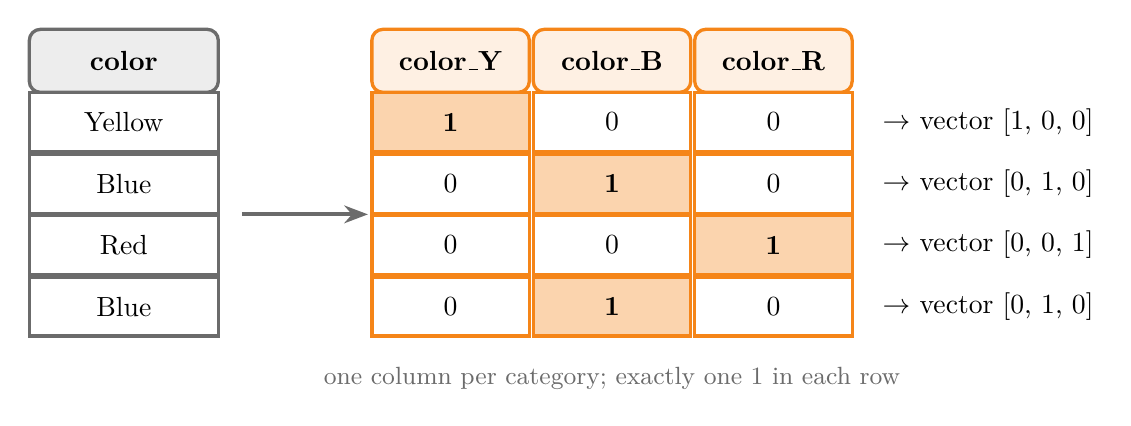
\begin{tikzpicture}
  % original column
  \node[box=cgrey, minimum width=2.4cm, minimum height=0.8cm, inner sep=3pt, font=\sffamily\bfseries] at (0,0) {color};
  \foreach \v [count=\i] in {Yellow,Blue,Red,Blue}
    \node[draw=cgrey, fill=white, minimum width=2.4cm, minimum height=0.75cm] at (0,-0.78*\i) {\v};
  \draw[arrow] (1.5,-1.95) -- (3.1,-1.95);
  % one-hot columns
  \foreach \h [count=\j] in {color\_Y, color\_B, color\_R}
    \node[box=corange, minimum width=2.0cm, minimum height=0.8cm, inner sep=3pt, font=\sffamily\bfseries] at (2.1+2.05*\j,0) {\h};
  \foreach \a/\b/\c [count=\i] in {1/0/0, 0/1/0, 0/0/1, 0/1/0} {
    \cell{4.15}{-0.78*\i}{\a}{\a}
    \cell{6.2}{-0.78*\i}{\b}{\b}
    \cell{8.25}{-0.78*\i}{\c}{\c}
    \node[anchor=west, font=\sffamily] at (9.5,-0.78*\i) {$\rightarrow$ vector [\a, \b, \c]};
  }
  \node[note, anchor=north] at (6.2,-3.75) {one column per category; exactly one 1 in each row};
\end{tikzpicture}
\end{document}
